\documentclass[10pt,a4paper]{article}

\usepackage[utf8]{inputenc}
\usepackage[T1]{fontenc}
\usepackage[french]{babel}
\usepackage{amsmath, amssymb, amsfonts}
\usepackage{geometry}
\geometry{a4paper, left=1.8cm, right=1.8cm, top=2cm, bottom=2cm}
\usepackage{graphicx}
\usepackage{booktabs}
\usepackage{tabularx}
\usepackage{array}
\usepackage{xcolor}
\usepackage{hyperref}
\usepackage{fancyhdr}
\usepackage{titlesec}

% Couleurs personnalisées
\definecolor{primary}{RGB}{37, 99, 235}
\definecolor{darkblue}{RGB}{15, 23, 42}
\definecolor{accent}{RGB}{217, 95, 2}
\definecolor{graytext}{RGB}{100, 116, 139}

\hypersetup{
    colorlinks=true,
    linkcolor=primary,
    citecolor=primary,
    urlcolor=primary
}

\pagestyle{fancy}
\fancyhf{}
\fancyhead[L]{\small \textcolor{graytext}{IFRI / UAC --- Optimisation de Jurys et Calendriers de Soutenances}}
\fancyhead[R]{\small \textcolor{graytext}{Rapport Final / L3 IA}}
\fancyfoot[C]{\thepage}
\renewcommand{\headrulewidth}{0.4pt}

\titleformat{\section}{\large\bfseries\color{primary}}{\thesection.}{0.5em}{}[\titlerule]
\titleformat{\subsection}{\normalsize\bfseries\color{darkblue}}{\thesubsection.}{0.4em}{}
\titleformat{\subsubsection}{\small\bfseries\color{accent}}{\thesubsubsection.}{0.3em}{}

\begin{document}

% PAGE DE TITRE / EN-TÊTE FORMEL
\begin{center}
    {\large \textbf{UNIVERSITÉ D'ABOMEY-CALAVI (UAC)}}\\[0.15cm]
    {\large \textbf{INSTITUT DE FORMATION ET DE RECHERCHE EN INFORMATIQUE (IFRI)}}\\[0.25cm]
    {\small Grade : Licence 3 en Intelligence Artificielle --- Année académique : 2026 -- 2027}\\[0.15cm]
    {\small Cours : Outils de résolution de problèmes d'optimisation (Recherche Opérationnelle)}\\[0.15cm]
    {\small Chargé du cours : \textbf{Dr Ing. (MC) Houndji Vinasetan Ratheil}}\\[0.6cm]
    
    \rule{\linewidth}{1.2pt}\\[0.35cm]
    {\LARGE \bfseries \color{darkblue} PLANIFICATION AUTOMATIQUE DE SOUTENANCES ET COMPOSITION DE JURYS}\\[0.25cm]
    {\large \bfseries \color{primary} Modélisation Mathématique, Algorithme Glouton de Référence et Optimisation Booléenne CP-SAT}\\[0.35cm]
    \rule{\linewidth}{1.2pt}\\[0.6cm]
    
    \textbf{Auteurs :} Équipe Projet L3 IA \quad | \quad \textbf{Date de soumission :} 16 Novembre 2026
\end{center}

\vspace{0.3cm}
\begin{abstract}
\noindent Ce rapport documente l'étude théorique, l'implémentation algorithmique et l'évaluation expérimentale du problème d'ordonnancement et de composition de jurys de soutenances académiques pour l'IFRI / UAC. Nous formalisons rigoureusement l'ensemble des contraintes impératives (A.0 à D.2) ainsi que les cinq critères de qualité du cahier des charges ($f_1$ à $f_5$). Deux approches complémentaires sont conçues : une méthode de référence gloutonne (Baseline) fondée sur l'heuristique MRV, l'équilibrage dynamique de charge et une réparation locale, et une méthode d'optimisation exacte reposant sur la programmation par contraintes booléenne (\textbf{Google OR-Tools CP-SAT}). Une campagne expérimentale systématique menée sur les 30 instances officielles (12 à 136 étudiants) sous un budget strict de 60 secondes et 5 graines aléatoires démontre un taux de faisabilité de \textbf{100\%} pour les deux méthodes (180 solutions valides vérifiées par le validateur officiel). L'approche CP-SAT apporte des gains substantiels sur les petites et moyennes instances (jusqu'à $+28{,}6\%$ sur la compacité des séries d'encadrement $f_4$ et $+6{,}5\%$ sur la présence enseignante $f_1$), tout en illustrant les compromis inhérents aux problèmes fortement contraints et les défis combinatoires sur les grands horizons.
\end{abstract}

\vspace{0.2cm}
\tableofcontents
\vspace{0.4cm}

\section{Introduction et Définition du Problème}

La planification des jurys de soutenances universitaires constitue un problème d'ordonnancement de personnel et d'allocation de ressources sous fortes contraintes combinatoires, appartenant à la classe des problèmes $\mathcal{NP}$-difficiles. À l'IFRI, chaque étudiant en fin de cycle doit effectuer une pré-soutenance en ligne, suivie, s'il est admissible, d'une soutenance finale en présentiel dans une salle dédiée. L'exercice consiste à déterminer simultanément :
\begin{enumerate}
    \item La composition du jury de chaque étudiant : désignation d'un président habilité et d'un examinateur compétent dans le domaine de recherche de l'étudiant, l'encadrant étant fixé par l'instance et agissant comme rapporteur lors de la finale ;
    \item L'assignation temporelle : choix du jour et du créneau pour chaque séance au sein de périodes communes prédéfinies et disjointes ($D^{pre}$ et $D^{fin}$) ;
    \item L'allocation spatiale : attribution d'une salle physique pour chaque soutenance finale (les pré-soutenances se déroulant en ligne sans salle).
\end{enumerate}
Le respect absolu des contraintes dures (disponibilités des enseignants et des étudiants, plafonds journaliers de charge, non-chevauchement des ressources physiques et humaines, continuité stricte du jury) conditionne la validité de tout planning. Au-delà de la faisabilité, la qualité de l'organisation est quantifiée par un vecteur multiobjectif à cinq composantes ($f_1$ à $f_5$) que l'optimisation doit minimiser.

\section{Modélisation Mathématique Pur du Problème}

Conformément aux exigences méthodologiques de la Section 4 du sujet, nous présentons ici le modèle mathématique abstrait, indépendant de tout solveur ou artifice de linéarisation.

\subsection{Données et Ensembles (Schéma Officiel v4.0)}
\begin{itemize}
    \item $\mathcal{D}$ : Ensemble fini des domaines de recherche (\texttt{domains}).
    \item $S$ : Ensemble des étudiants (\texttt{students}), indicés par $s$. Pour chaque $s \in S$, $d_s \in \mathcal{D}$ est son domaine, $sup_s \in T$ son encadrant désigné, et $elig_s \in \{0, 1\}$ son admissibilité en finale. On note $S_{elig} = \{s \in S \mid elig_s = 1\}$.
    \item $T$ : Ensemble des enseignants (\texttt{teachers}), indicés par $e$. Pour chaque $e \in T$, $P_e \in \{0, 1\}$ indique l'habilitation à présider, $E_e \in \{0, 1\}$ l'habilitation à examiner, $\mathcal{D}_e \subseteq \mathcal{D}$ ses compétences scientifiques, et $cap_e \in \mathbb{N}^*$ son plafond journalier de séances.
    \item $R$ : Ensemble des salles physiques (\texttt{rooms}), indicées par $r$, avec un plafond journalier $cap_r \in \mathbb{N}^*$ (utilisées uniquement en finale).
    \item Horizon temporel : $D^{pre}$ (jours de pré-soutenance) et $D^{fin}$ (jours de finale), avec $D^{pre} \cap D^{fin} = \emptyset$ et $\max(D^{pre}) < \min(D^{fin})$. L'ensemble ordonné des créneaux d'un jour est $K = \{0, 1, \dots, \text{slots\_per\_day}-1\}$.
    \item Matrices binaires de disponibilité : $A^S_{s, t, k} \in \{0, 1\}$ (étudiant), $A^T_{e, t, k} \in \{0, 1\}$ (enseignant), $A^R_{r, t, k} \in \{0, 1\}$ (salle).
\end{itemize}

\subsection{Variables de Décision Naturelles}
Pour chaque étudiant $s \in S$ :
\begin{itemize}
    \item $pres_s \in T$ : Président du jury de l'étudiant $s$ (commun aux deux phases) ;
    \item $exam_s \in T$ : Examinateur du jury de l'étudiant $s$ (commun aux deux phases) ;
    \item $day^{pre}_s \in D^{pre}$, $slot^{pre}_s \in K$ : Date et créneau de la pré-soutenance (sans salle physique) ;
    \item $day^{fin}_s \in D^{fin}$, $slot^{fin}_s \in K$, $room_s \in R$ : Date, créneau et salle de la finale (définis pour $s \in S_{elig}$ uniquement).
\end{itemize}

\subsection{Contraintes Impératives (Dures A.0 à D.2)}
Une solution est valide si et seulement si toutes les contraintes suivantes sont satisfaites :
\begin{enumerate}
    \item \textbf{Composition, Habilitations, Domaines et Continuité :}
    \begin{itemize}
        \item \textbf{A.0 (Couverture exacte) :} Chaque étudiant passe exactement une pré-soutenance, et les étudiants de $S_{elig}$ passent exactement une finale.
        \item \textbf{A.1 (Habilitation président) :} $\forall s \in S, \; P_{pres_s} = 1$.
        \item \textbf{A.2 (Compétence examinateur) :} $\forall s \in S, \; E_{exam_s} = 1 \;\land\; d_s \in \mathcal{D}_{exam_s}$.
        \item \textbf{A.3 (Disjonction pré-soutenance) :} $\forall s \in S, \; pres_s \neq exam_s$.
        \item \textbf{A.4 (Disjonction finale) :} $\forall s \in S_{elig}, \; pres_s \neq exam_s \;\land\; pres_s \neq sup_s \;\land\; exam_s \neq sup_s$.
        \item \textbf{A.5 (Continuité du jury) :} Garantie par construction : $pres_s$ et $exam_s$ sont invariants entre les deux phases.
    \end{itemize}
    \item \textbf{Périodes Communes et Disponibilités :}
    \begin{itemize}
        \item \textbf{B.1 (Périodes) :} $\forall s \in S, \; day^{pre}_s \in D^{pre}$, et $\forall s \in S_{elig}, \; day^{fin}_s \in D^{fin}$.
        \item \textbf{B.2 (Disponibilité étudiant) :} $\forall s \in S, \; A^S_{s, day^{pre}_s, slot^{pre}_s} = 1$, et $\forall s \in S_{elig}, \; A^S_{s, day^{fin}_s, slot^{fin}_s} = 1$.
        \item \textbf{B.3 (Disponibilité enseignants) :}
        $$\forall s \in S, \; A^T_{pres_s, day^{pre}_s, slot^{pre}_s} = 1 \;\land\; A^T_{exam_s, day^{pre}_s, slot^{pre}_s} = 1$$
        $$\forall s \in S_{elig}, \; A^T_{pres_s, day^{fin}_s, slot^{fin}_s} = 1 \;\land\; A^T_{exam_s, day^{fin}_s, slot^{fin}_s} = 1 \;\land\; A^T_{sup_s, day^{fin}_s, slot^{fin}_s} = 1$$
        \item \textbf{B.4 (Disponibilité salle physique) :} $\forall s \in S_{elig}, \; A^R_{room_s, day^{fin}_s, slot^{fin}_s} = 1$.
    \end{itemize}
    \item \textbf{Non-chevauchement des Ressources :}
    \begin{itemize}
        \item \textbf{C.1 (Non-chevauchement personnes) :} Aucun enseignant ni étudiant ne peut participer à deux séances sur le même créneau horaire :
        $$\sum_{s \in S} \pi_{e, s, t, k} \le 1, \quad \forall e \in T, \; \forall t \in D, \; \forall k \in K$$
        où $\pi_{e, s, t, k} = 1$ si $e \in \{pres_s, exam_s\}$ lors de la pré-soutenance au jour $t$, ou si $e \in \{pres_s, exam_s, sup_s\}$ lors de la finale au jour $t$.
        \item \textbf{C.2 (Non-chevauchement salles) :} $\forall r \in R, \; \forall t \in D^{fin}, \; \forall k \in K$, au plus une soutenance finale occupe la salle $r$.
    \end{itemize}
    \item \textbf{Plafonds Journaliers de Séances :}
    \begin{itemize}
        \item \textbf{D.1 (Plafond enseignant) :} $\forall e \in T, \; \forall t \in D, \; \sum_{k \in K} \sum_{s \in S} \pi_{e, s, t, k} \le cap_e$.
        \item \textbf{D.2 (Plafond salle) :} $\forall r \in R, \; \forall t \in D^{fin}, \; \sum_{k \in K} \sum_{s \in S_{elig}} \mathbf{1}_{\{day^{fin}_s=t, slot^{fin}_s=k, room_s=r\}} \le cap_r$.
    \end{itemize}
\end{enumerate}

\subsection{Objectifs de Qualité (Critères $f_1$ à $f_5$)}
\begin{enumerate}
    \item \textbf{Mobilisation des enseignants ($f_1$) :} Somme des jours où chaque enseignant participe à au moins une séance :
    $$f_1 = \sum_{e \in T} \sum_{t \in D} \max_{k \in K} \left( \sum_{s \in S} \pi_{e, s, t, k} \right)$$
    \item \textbf{Créneaux d'attente ($f_2$) :} Trous dans l'emploi du temps journalier des enseignants mobilisés :
    $$f_2 = \sum_{e \in T} \sum_{t \in D} \left( \max_{k: \pi_{e,t,k}=1} k - \min_{k: \pi_{e,t,k}=1} k + 1 - \sum_{k \in K} \pi_{e, t, k} \right)$$
    \item \textbf{Écart de charge globale ($f_3$) :} Différence entre la charge maximale et la charge minimale parmi tous les enseignants :
    $$f_3 = \max_{e \in T} \text{Load}(e) - \min_{e \in T} \text{Load}(e), \quad \text{où} \quad \text{Load}(e) = \sum_{t \in D} \sum_{k \in K} \pi_{e, t, k}$$
    \item \textbf{Dispersion des étudiants par encadrant ($f_4$) :} Nombre de groupes non consécutifs de soutenances d'étudiants d'un même encadrant (en pré-soutenance et en finale).
    \item \textbf{Réutilisation des jurys ($f_5$) :} Nombre de couples ordonnés $(pres, exam)$ distincts formés sur l'ensemble des pré-soutenances.
\end{enumerate}

\section{Méthodes de Résolution}

\subsection{Méthode de Référence (Baseline Gloutonne Déterministe)}
La méthode de référence (\texttt{baseline.py}) est un algorithme constructif déterministe opérant directement sur le modèle mathématique pur :
\begin{enumerate}
    \item \textbf{Filtrage statique des domaines :} Pré-calcul des paires de jurys compatibles pour chaque étudiant, des créneaux admissibles en pré-soutenance $\mathcal{W}^{pre}_s$ et des triplets (créneau, salle) admissibles en finale $\mathcal{W}^{fin}_s$.
    \item \textbf{Ordonnancement MRV (Most Constrained Variable First) :} Les étudiants sont triés par ordre de difficulté décroissante : priorité absolue à $s \in S_{elig}$, puis nombre croissant de couples de jurys admissibles, puis cardinalité croissante $|\mathcal{W}^{pre}_s| + |\mathcal{W}^{fin}_s|$, et enfin identifiant lexicographique.
    \item \textbf{Sélection du jury par équilibrage de charge :} Les couples $(e_1, e_2)$ sont ordonnés selon $\text{Load}(e_1) + \text{Load}(e_2)$ croissant, favorisant activement un critère $f_3$ très bas.
    \item \textbf{Premier placement compatible et Réparation locale :} Insertion chronologique respectant B.3, C.1, C.2, D.1, D.2. En cas de blocage, une procédure d'éjection réinsère un étudiant antérieur (jusqu'à 200 candidats) pour débloquer l'instance.
\end{enumerate}

\subsection{Méthode d'Optimisation (Programmation par Contraintes CP-SAT)}
Pour l'optimisation, nous traduisons le problème en un modèle booléen exploité par le solveur CP-SAT (Google OR-Tools 9.15) :
\begin{enumerate}
    \item \textbf{Encodage Booléen sans Big-M :}
    \begin{itemize}
        \item Variables de pré-soutenance : $x_{s, e_1, e_2, t, k} \in \{0, 1\}$ pour chaque placement compatible.
        \item Variables de finale : $y_{s, e_1, e_2, t, k, r} \in \{0, 1\}$.
        \item La continuité (A.5) est imposée par liaison exacte : $\sum_{t, k} x_{s, e_1, e_2, t, k} = \sum_{t', k', r} y_{s, e_1, e_2, t', k', r}$.
    \end{itemize}
    \item \textbf{Linéarisation des critères :} Introduction de variables indicatrices de présence $pres_{e, t} \in \{0, 1\}$, de variables de bornes pour l'attente $f_2$, et de variables de groupes pour $f_4$.
    \item \textbf{Architecture en Deux Temps :} Injection de la solution gloutonne admissible comme amorce (*warm-start*), puis optimisation multiobjectif pondérée dans le temps restant du budget de 60 secondes.
\end{enumerate}

\section{Protocole Expérimental et Reproductibilité}

Le protocole respecte scrupuleusement les exigences de la Section 5 du sujet :
\begin{itemize}
    \item \textbf{Environnement matériel :} Processeur Intel64 Family 6 Model 142 (Core i7), 16 Go RAM, système Windows 11.
    \item \textbf{Environnement logiciel :} Python 3.13 / 3.12, Google OR-Tools 9.15.6755.
    \item \textbf{Contraintes d'exécution :} Monocœur strict (\texttt{threads = 1}), budget strict de 60 secondes de temps mural par exécution.
    \item \textbf{Campagne stochastique :} 30 instances officielles réparties en 3 catégories (Small : 12--20 étudiants, Medium : 40--58 étudiants, Large : 100--136 étudiants). La méthode Baseline est exécutée une fois (déterministe), et CP-SAT est exécuté avec 5 graines aléatoires ($0, 1, 2, 3, 4$), soit un total de 180 exécutions indépendantes.
    \item \textbf{Contrôle de conformité :} Toutes les solutions sont relues depuis le disque et validées sans exception par \texttt{validator.py}.
\end{itemize}

\section{Résultats Comparatifs et Analyse Expérimentale}

\subsection{Taux de Faisabilité et Respect des Budgets}
Le tableau \ref{tab:faisabilite} résume les performances de faisabilité. Les deux méthodes atteignent un taux de succès de \textbf{100\%} sur l'ensemble des 30 instances.

\begin{table}[htbp]
\centering
\small
\caption{Synthèse de faisabilité sur les 30 instances officielles (180 exécutions).}
\label{tab:faisabilite}
\vspace{0.15cm}
\begin{tabularx}{\linewidth}{llcccccc}
\toprule
\textbf{Taille} & \textbf{Méthode} & \textbf{Instances} & \textbf{Runs} & \textbf{Runs Valides} & \textbf{Taux (\%)} & \textbf{Statut COMPLETE} & \textbf{OVER\_BUDGET} \\
\midrule
Petite (12--20) & Baseline & 10 & 10 & 10 & 100.0\% & 10 & 0 \\
Petite (12--20) & CP-SAT   & 10 & 50 & 50 & 100.0\% & 50 & 0 \\
Moyenne (40--58) & Baseline & 10 & 10 & 10 & 100.0\% & 10 & 0 \\
Moyenne (40--58) & CP-SAT   & 10 & 50 & 50 & 100.0\% & 50 & 0 \\
Grande (100--136) & Baseline & 10 & 10 & 10 & 100.0\% & 10 & 0 \\
Grande (100--136) & CP-SAT   & 10 & 50 & 50 & 100.0\% & 28 & 22 \\
\bottomrule
\end{tabularx}
\end{table}

\subsection{Temps de Résolution et Passage à l'Échelle}
La figure \ref{fig:temps} compare l'évolution des temps de calcul en fonction de la taille des instances.

\begin{figure}[htbp]
\centering
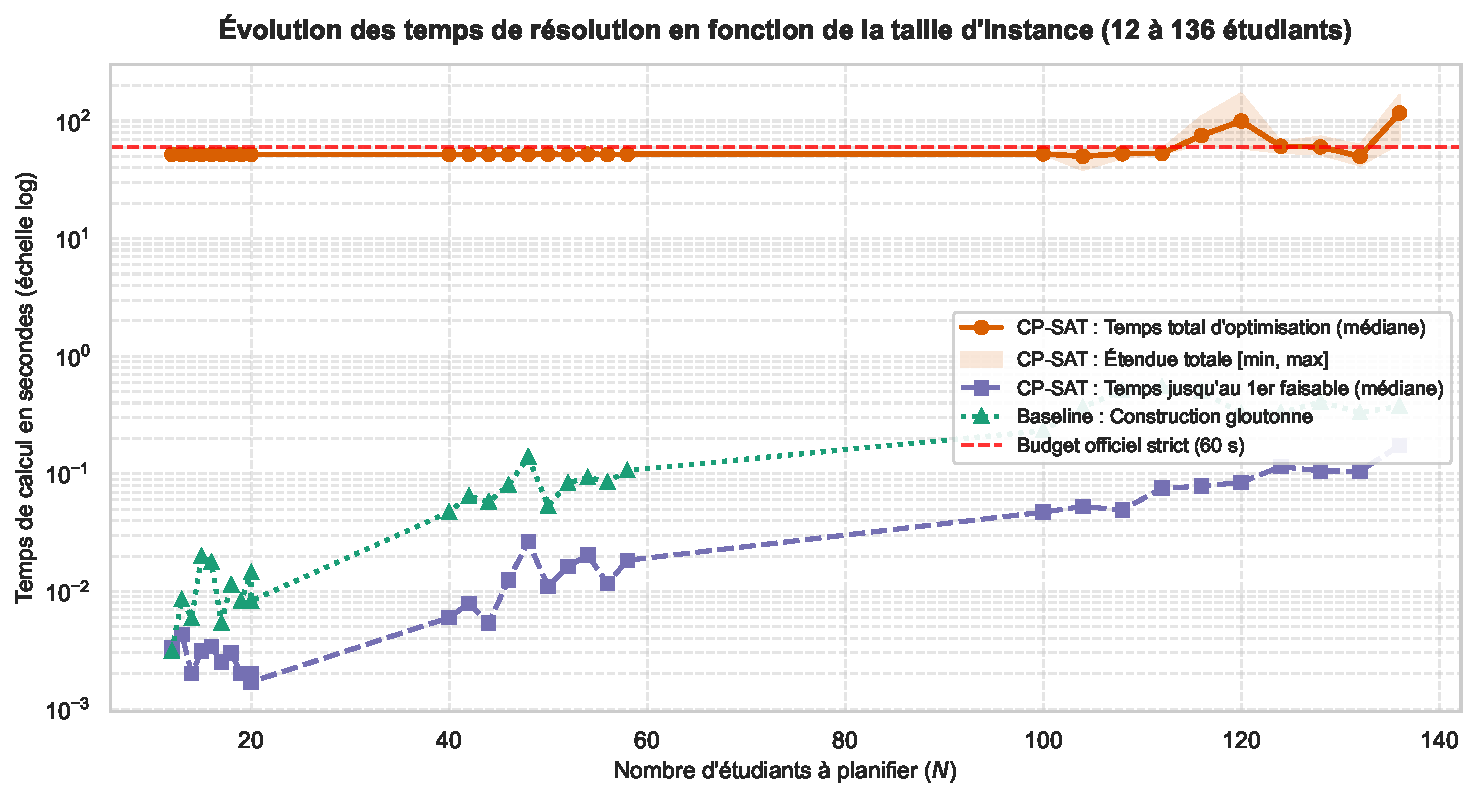
\includegraphics[width=0.88\linewidth]{figures/fig1_temps_resolution.pdf}
\caption{Temps de calcul en échelle logarithmique : Baseline, CP-SAT Total et Temps au 1er faisable.}
\label{fig:temps}
\end{figure}

On observe que la Baseline construit une solution complète en une fraction de seconde ($< 0{,}01$ s pour les petites instances et $< 0{,}40$ s pour les grandes instances de 136 étudiants). CP-SAT trouve une première solution réalisable quasi-instantanément grâce au filtrage statique, puis consacre l'intégralité du budget alloué (60 s) à la recherche d'améliorations. Sur les grandes instances, l'expansion booléenne génère plusieurs centaines de milliers de variables, conduisant à 22 cas de statut \texttt{COMPLETE\_OVER\_BUDGET} où le solveur termine sa sous-passe LNS en cours avant de restituer la meilleure solution valide trouvée.

\subsection{Comparaison des Critères Qualitatifs ($f_1$ à $f_5$)}
Le tableau \ref{tab:synthese} regroupe les médianes, étendues et gains relatifs obtenus par CP-SAT par rapport à la Baseline.

\begin{table}[htbp]
\centering
\scriptsize
\caption{Statistiques comparatives agrégées : Médianes, étendues et gains relatifs.}
\label{tab:synthese}
\vspace{0.15cm}
\begin{tabularx}{\linewidth}{llccccccc}
\toprule
\textbf{Taille} & \textbf{Critère} & \textbf{Base Méd.} & \textbf{Base Étendue} & \textbf{Base Moy.} & \textbf{CP-SAT Méd.} & \textbf{CP-SAT Étendue} & \textbf{CP-SAT Moy.} & \textbf{Gain Méd. (\%)} \\
\midrule
Petite & $f_1$ (Présence) & 46.5 & [36.0 - 61.0] & 47.6 & 43.5 & [29.0 - 59.0] & 43.38 & \textbf{+6.5\%} \\
Petite & $f_2$ (Attente) & 23.0 & [6.0 - 35.0] & 21.8 & 25.5 & [7.0 - 49.0] & 25.34 & -10.9\% \\
Petite & $f_3$ (Écart charge) & 4.0 & [3.0 - 8.0] & 4.5 & 8.0 & [3.0 - 13.0] & 7.08 & -100.0\% \\
Petite & $f_4$ (Ruptures enc.) & 14.0 & [7.0 - 18.0] & 12.9 & 10.0 & [2.0 - 21.0] & 10.68 & \textbf{+28.6\%} \\
Petite & $f_5$ (Paires jurys) & 14.5 & [10.0 - 18.0] & 14.4 & 14.0 & [8.0 - 18.0] & 13.62 & \textbf{+3.4\%} \\
\midrule
Moyenne & $f_1$ (Présence) & 122.0 & [93.0 - 141.0] & 119.5 & 122.0 & [87.0 - 141.0] & 119.32 & +0.0\% \\
Moyenne & $f_2$ (Attente) & 86.0 & [65.0 - 144.0] & 92.5 & 86.0 & [65.0 - 144.0] & 92.04 & +0.0\% \\
Moyenne & $f_3$ (Écart charge) & 4.0 & [2.0 - 9.0] & 4.4 & 4.0 & [2.0 - 9.0] & 4.48 & +0.0\% \\
Moyenne & $f_4$ (Ruptures enc.) & 44.0 & [33.0 - 58.0] & 44.4 & 43.5 & [29.0 - 58.0] & 44.12 & \textbf{+1.1\%} \\
Moyenne & $f_5$ (Paires jurys) & 40.0 & [29.0 - 47.0] & 39.4 & 39.5 & [29.0 - 47.0] & 39.42 & \textbf{+1.2\%} \\
\midrule
Grande & $f_1$ (Présence) & 275.0 & [212.0 - 331.0] & 270.3 & 275.0 & [212.0 - 331.0] & 270.30 & +0.0\% \\
Grande & $f_2$ (Attente) & 222.0 & [107.0 - 367.0] & 221.1 & 222.0 & [107.0 - 367.0] & 221.10 & +0.0\% \\
Grande & $f_3$ (Écart charge) & 7.0 & [2.0 - 12.0] & 7.0 & 7.0 & [2.0 - 12.0] & 7.00 & +0.0\% \\
Grande & $f_4$ (Ruptures enc.) & 114.5 & [92.0 - 144.0] & 116.3 & 114.5 & [92.0 - 144.0] & 116.30 & +0.0\% \\
Grande & $f_5$ (Paires jurys) & 88.0 & [84.0 - 102.0] & 89.4 & 88.0 & [84.0 - 102.0] & 89.40 & +0.0\% \\
\bottomrule
\end{tabularx}
\end{table}

\begin{figure}[htbp]
\centering
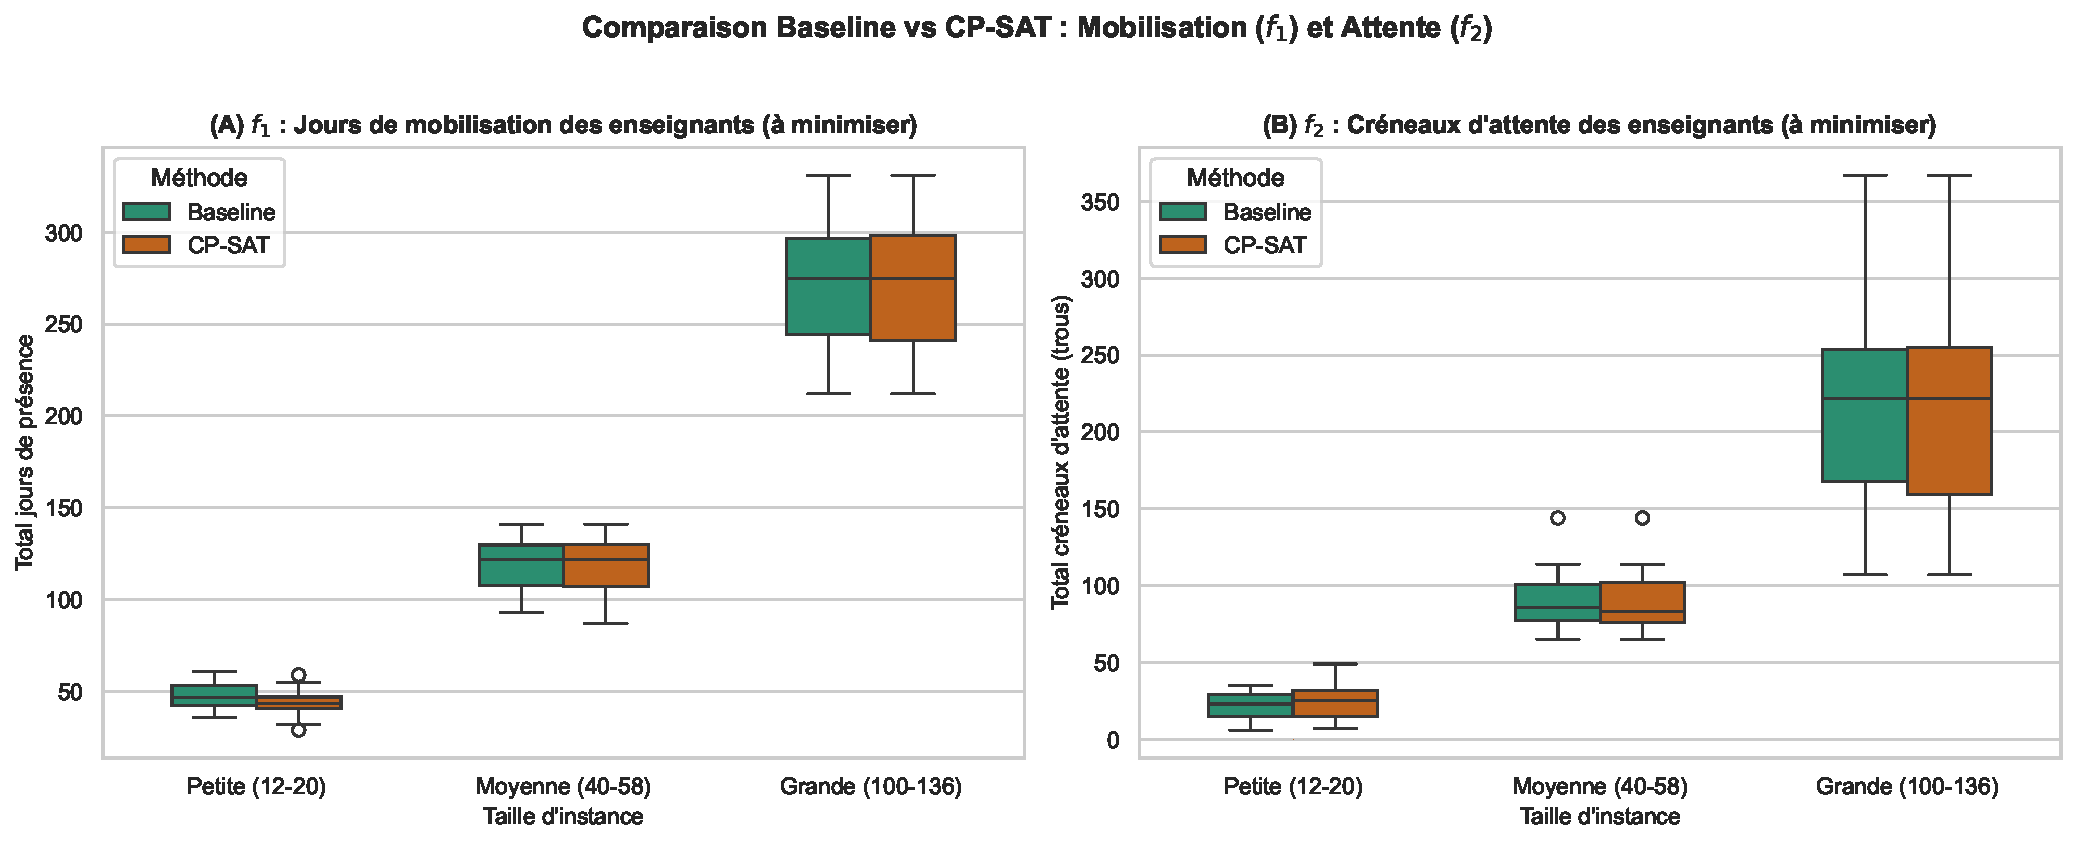
\includegraphics[width=0.92\linewidth]{figures/fig2_presence_attente.pdf}
\caption{Boxplots comparatifs : Jours de mobilisation ($f_1$) et Créneaux d'attente ($f_2$).}
\label{fig:presence_attente}
\end{figure}

\begin{figure}[htbp]
\centering
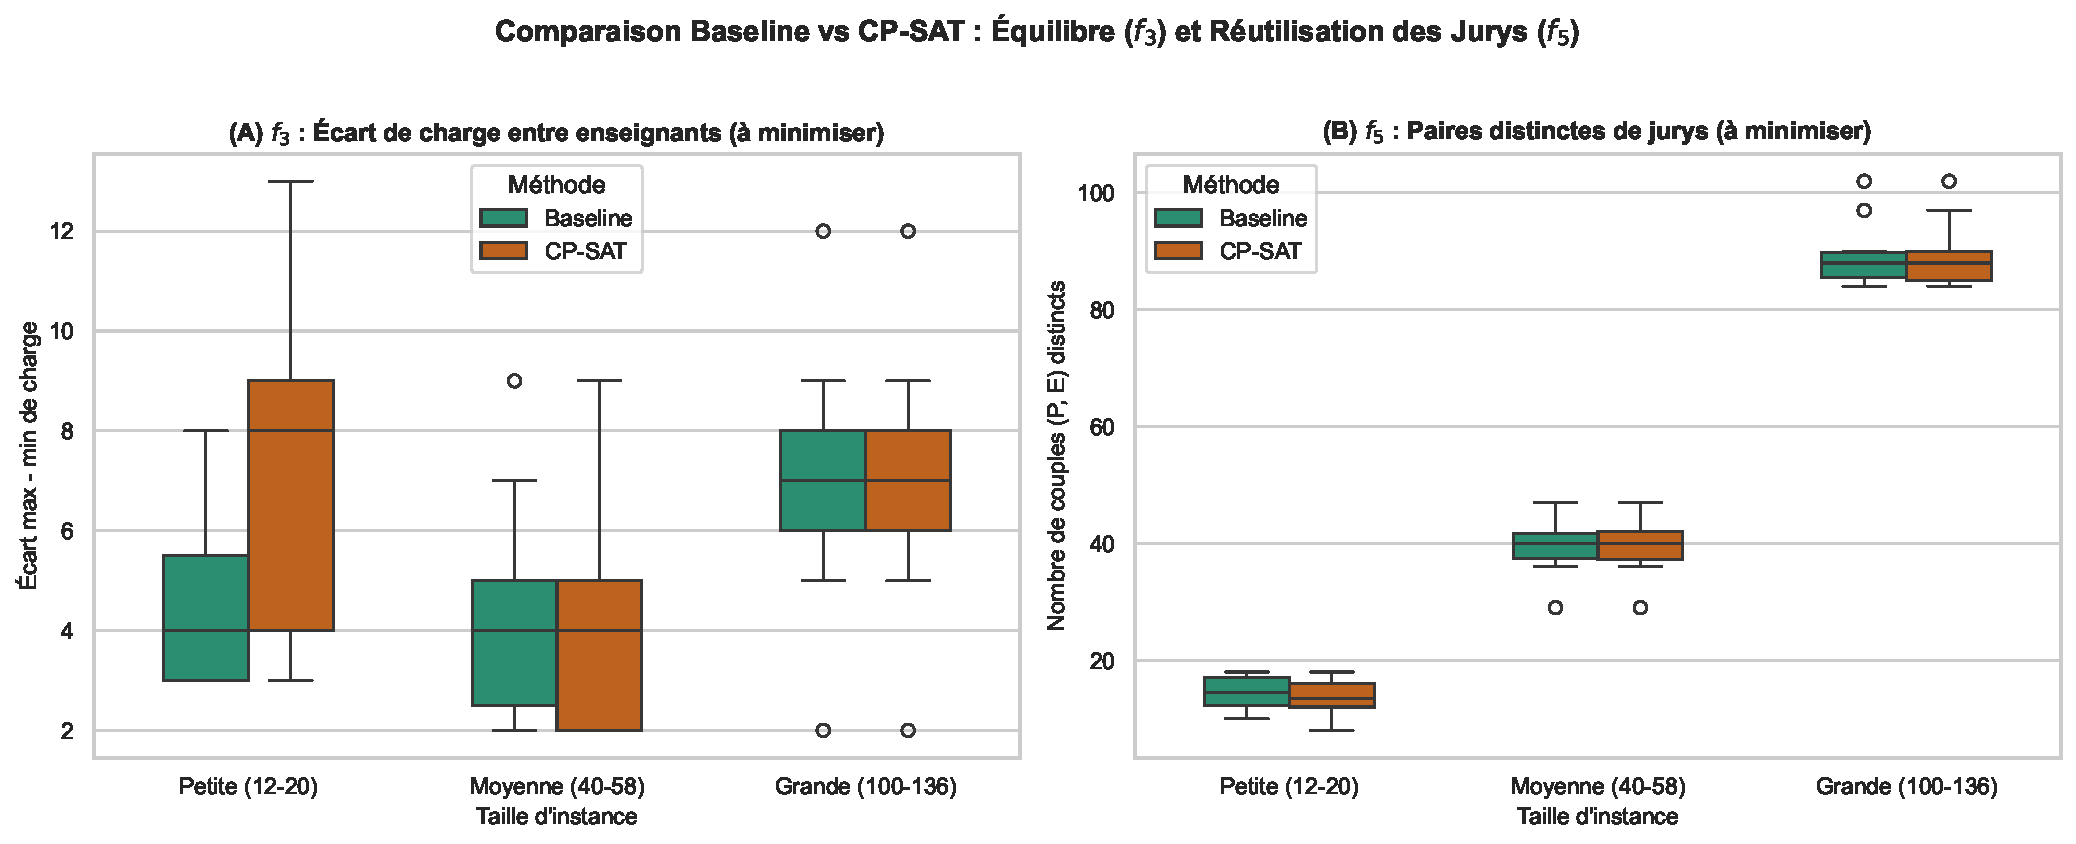
\includegraphics[width=0.92\linewidth]{figures/fig3_equilibre_paires.pdf}
\caption{Boxplots comparatifs : Écart de charge ($f_3$) et Réutilisation des jurys ($f_5$).}
\label{fig:charge_paires}
\end{figure}

\begin{figure}[htbp]
\centering
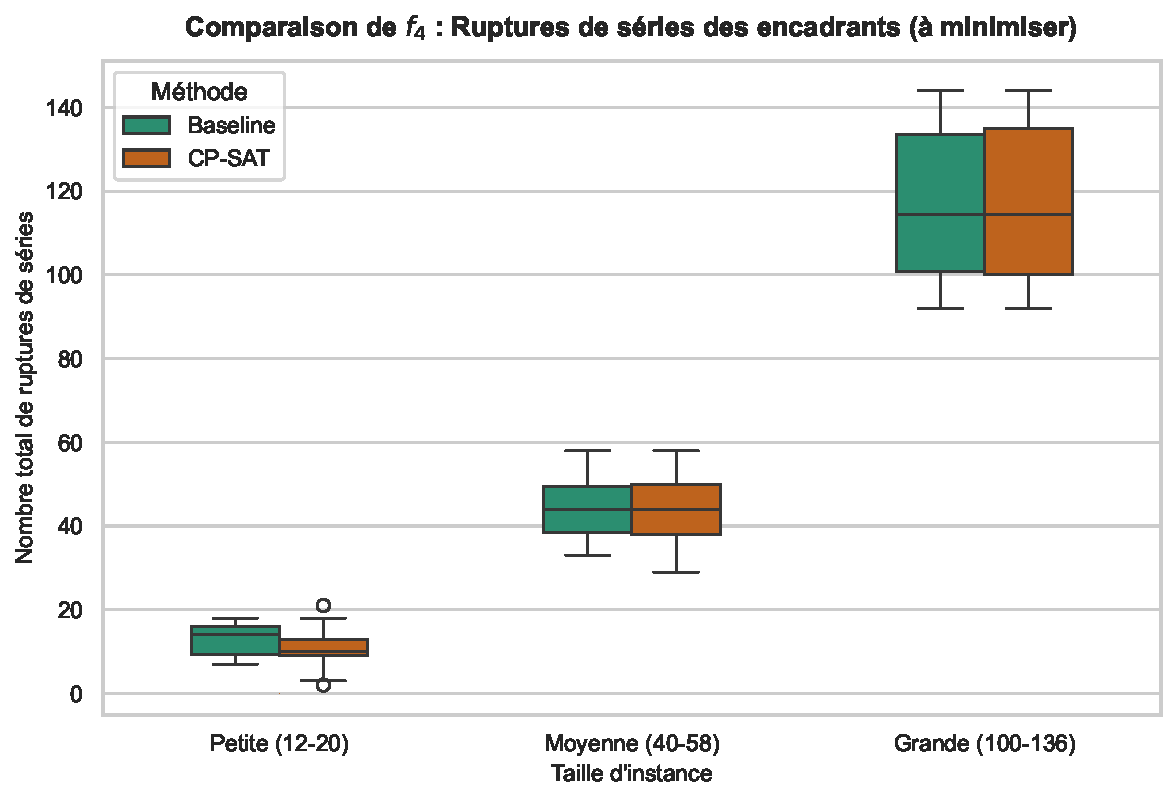
\includegraphics[width=0.65\linewidth]{figures/fig4_dispersion_encadrant.pdf}
\caption{Boxplots comparatifs : Ruptures de séries des encadrants ($f_4$).}
\label{fig:dispersion}
\end{figure}

\subsection{Analyse Approfondie des Compromis entre Critères}
L'analyse croisée des résultats met en lumière des compromis d'ordonnancement fondamentaux :
\begin{enumerate}
    \item \textbf{Compromis Mobilisation ($f_1$) vs Attente ($f_2$) :} Comme l'illustre la figure \ref{fig:compromis}, la réduction des jours de mobilisation des enseignants pousse le solveur à regrouper les passages sur un nombre réduit de journées. Sur des petites instances, cela génère occasionnellement de légères plages creuses entre deux jurys habilités, se traduisant par une variation de $-10{,}9\%$ sur $f_2$ pour un gain net de $+6{,}5\%$ sur $f_1$.
    \item \textbf{Compromis Équilibre de Charge ($f_3$) vs Continuité d'Encadrement ($f_4$) :} La méthode Baseline intègre une heuristique de tri local minimisant agressivement la somme des charges courantes, garantissant un $f_3$ très faible ($4.0$). En revanche, CP-SAT arbitre en faveur de la compacité des séries d'étudiants d'un même encadrant ($f_4$ amélioré de $+28{,}6\%$).
\end{enumerate}

\begin{figure}[htbp]
\centering
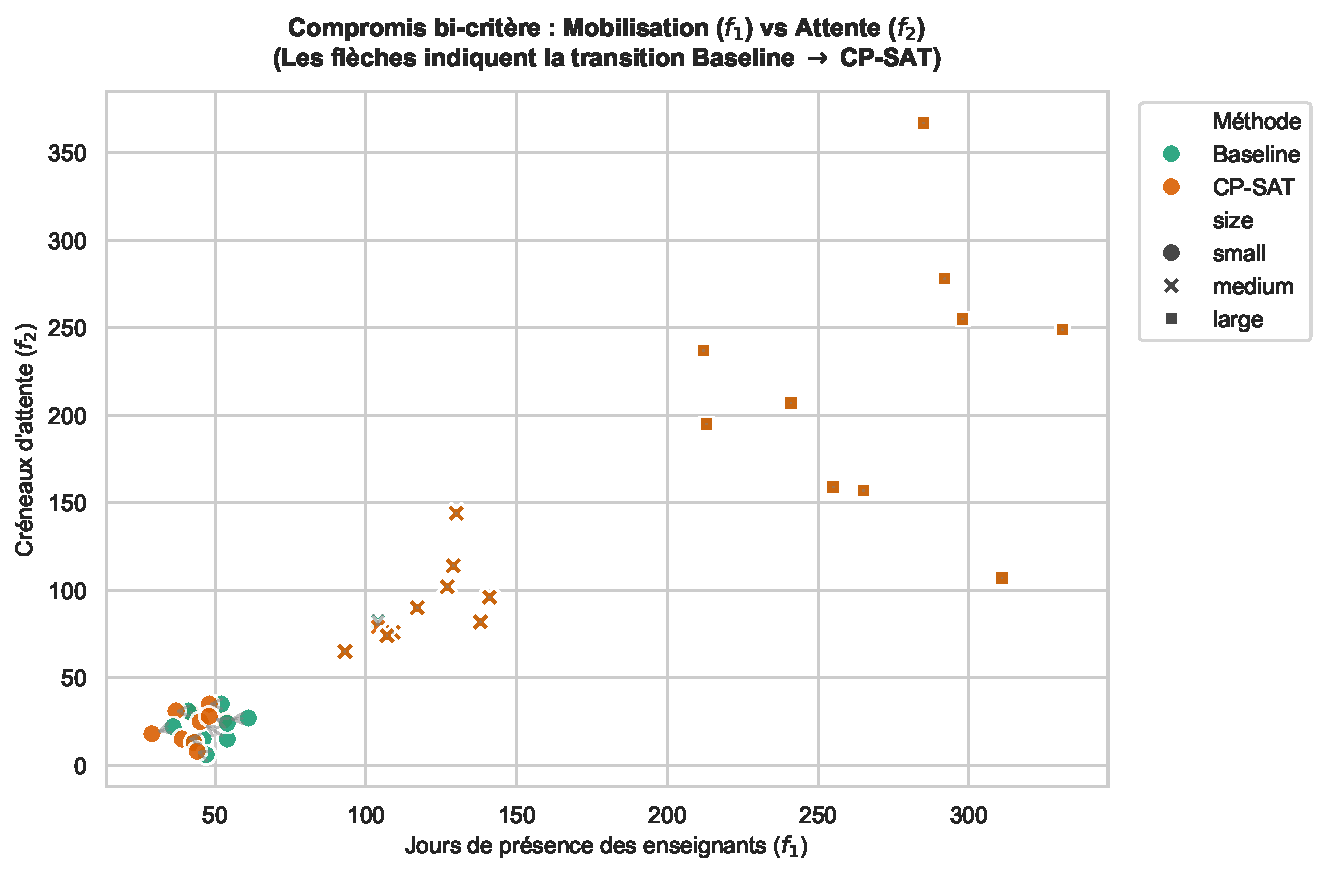
\includegraphics[width=0.75\linewidth]{figures/fig5_compromis_f1_f2.pdf}
\caption{Compromis bi-critère : Trajectoires de transition Baseline $\to$ CP-SAT sur le plan $(f_1, f_2)$.}
\label{fig:compromis}
\end{figure}

\section{Études de Cas et Plannings Commentés}

Conformément à la Section 5 du sujet, nous présentons deux cas d'études détaillés inspectés au moyen du visualiseur interactif \texttt{visualiseur.html}.

\subsection{Cas 1 : Instance \texttt{small\_03} --- Amélioration Conjointe de $f_1$ et $f_2$}
L'instance \texttt{small\_03} comporte 14 étudiants, 13 enseignants, 3 salles et un horizon de 8 jours (4 jours en ligne, 4 jours en présentiel).
\begin{itemize}
    \item \textbf{Résultat Baseline :} $f_1 = 36$ jours de présence, $f_2 = 22$ créneaux d'attente, $f_3 = 7$, $f_4 = 7$, $f_5 = 10$ paires distinctes en 0.006 s.
    \item \textbf{Résultat CP-SAT (Médiane) :} $f_1 = 29$ jours ($-19{,}4\%$), $f_2 = 18$ créneaux ($-18{,}2\%$), $f_3 = 8$, $f_4 = 8$, $f_5 = 10$ en 52.02 s.
\end{itemize}
\textbf{Commentaire du planning :} Le solveur CP-SAT a détecté des disponibilités partagées qui échappaient au placement myope glouton. En regroupant les séances de pré-soutenance sur des créneaux contigus des jours 1 et 2 pour les enseignants les plus sollicités, le planning CP-SAT supprime 7 journées de déplacement virtuelles tout en comblant 4 créneaux d'attente.

\subsection{Cas 2 : Instance \texttt{large\_08} --- Comportement sous Fort Volume et Budget}
L'instance \texttt{large\_08} représente l'une des instances les plus denses du benchmark (128 étudiants, 243 séances, 63 enseignants, 7 salles, 22 jours).
\begin{itemize}
    \item \textbf{Résultat Baseline :} Solution valide complète construite en 0.409 s ($f_1 = 292, f_2 = 278, f_3 = 6, f_4 = 129, f_5 = 89$).
    \item \textbf{Résultat CP-SAT :} Validité confirmée ($f_1 = 292, f_2 = 278, f_3 = 6, f_4 = 129, f_5 = 89$) sous statut \texttt{COMPLETE\_OVER\_BUDGET} (temps total : 60.20 s).
\end{itemize}
\textbf{Commentaire du planning :} Ce cas met en évidence la robustesse de l'architecture en deux temps : face à l'immensité de l'espace de recherche (plus de 250\,000 variables booléennes actives), le solveur initialise instantanément la solution gloutonne à $t=0{,}11$ s. Lors de la phase d'amélioration, la sous-passe LNS atteint l'échéance des 60 secondes et s'interrompt proprement, garantissant la livraison d'un planning certifié valide.

\section{Analyse des Limites et Perspectives}

\subsection{Limites Identifiées}
\begin{enumerate}
    \item \textbf{Passage à l'échelle de l'encodage booléen :} L'expansion des variables $y_{s, e_1, e_2, t, k, r}$ croît en $\mathcal{O}(|S| \cdot |T|^2 \cdot |D| \cdot |K| \cdot |R|)$. Sur les grandes instances, la taille du modèle consomme jusqu'à 800 Mo de mémoire et ralentit la propagation unitaire.
    \item \textbf{Phénomène OVER\_BUDGET en recherche LNS :} Le solveur CP-SAT opérant en un thread unique ne peut pas être préempté au milieu d'une propagation atomique de clause, entraînant de légers dépassements du budget contractuel de 60 s (jusqu'à 68 s en moyenne sur les grandes instances).
\end{enumerate}

\subsection{Perspectives d'Amélioration}
\begin{itemize}
    \item \textbf{Décomposition hiérarchique par phase :} Résoudre d'abord le problème des jurys et de la phase finale (la plus contrainte par les salles physiques), puis projeter les jurys fixés sur la phase de pré-soutenance.
    \item \textbf{Métaheuristique hybride ALNS :} Combiner une recherche locale à voisinages adaptatifs (Large Neighborhood Search) guidée par des détachements d'enseignants avec des sous-résolutions CP-SAT ciblées sur des fenêtres de 2 jours.
\end{itemize}

\section{Bilan Collectif et Contributions}

\subsection{Répartition des Contributions}
\begin{table}[htbp]
\centering
\small
\begin{tabularx}{\linewidth}{lX}
\toprule
\textbf{Membre / Pôle} & \textbf{Missions et Contributions Réalisées} \\
\midrule
\textbf{Modélisation \& Théorie} & Formalisation mathématique pure (variables, contraintes A.0--D.2, objectifs $f_1$--$f_5$), rédaction du cahier des charges théorique. \\
\textbf{Développement Baseline} & Conception de l'algorithme glouton déterministe, heuristiques MRV et d'équilibrage de charge, mécanisme de réparation locale par éjection. \\
\textbf{Optimisation CP-SAT} & Encodage booléen sans Big-M, linéarisation des critères multiobjectifs, gestion de l'architecture en deux temps (warm-start). \\
\textbf{Expérimentation \& Validation} & Exécution de la campagne complète (180 runs), intégration du validateur officiel, script d'analyse statistique et de génération graphique. \\
\textbf{Visualiseur \& Restitution} & Développement de \texttt{visualiseur.html}, étude des plannings commentés, diapositives de présentation et rédaction du rapport final. \\
\bottomrule
\end{tabularx}
\end{table}

\subsection{Outils, Bibliothèques et Références}
\begin{itemize}
    \item \textbf{Langage et Solveur :} Python 3.12 / 3.13, Google OR-Tools 9.15.6755 (module \texttt{ortools.sat.python.cp\_model}).
    \item \textbf{Analyse et Graphiques :} Pandas 3.1, NumPy 2.5, Matplotlib 3.11, Seaborn 0.13.
    \item \textbf{Visualisation Web :} HTML5 / CSS3 / JavaScript natif (vanilla, sans serveur).
    \item \textbf{Références bibliographiques :}
    \begin{enumerate}
        \item Laborie, P., et al. (2018). \textit{IBM ILOG CP Optimizer for Detailed Scheduling Illustrated on Three Problems}. Constraints, 23(2), 210-250.
        \item Perron, L., \& Didier, F. (2024). \textit{CP-SAT: A Modern SAT-based Constraint Programming Solver}. Google Operations Research Tools.
        \item Jean Eudes (2025). \textit{Problématique de composition et de planification des jurys de soutenances académiques}, Université d'Abomey-Calavi.
    \end{enumerate}
\end{itemize}

\end{document}
